\section{Theoretical and Simulation Analysis}
\label{sec:analysis}

In this stage we are going to compare the theoretical and simulation analysis, but first we are going to present each part of the circuit by its self and discuss how it works. The constant values in the table below were the ones we used for this activity.

\begin{table}[h]
    \centering
    \begin{tabular}{|l|c|c|}
    \hline
    {\bf Name} & {\bf Value} & {\bf Units} \\ \hline
    $R_1$ & $1000$ & $\Omega$ [Ohms] \\ \hline
    $R_2$ & $1000$ & $\Omega$ [Ohms] \\ \hline
    $R_3$ & $100000$ & $\Omega$ [Ohms] \\ \hline
    $R_4$ & $1000$ & $\Omega$ [Ohms] \\ \hline
    $C_1$ & $220$ & $\eta F$ [$\eta$Farads]\\ \hline
    $C_2$ & $110$ & $\eta F$ [$\eta$Farads] \\ \hline
    \end{tabular}
    \caption[Constants Values]{Constants Values}
    \label{tab:constants}
\end{table}


\subsection{High Pass Stage}
\label{subsec:stat}
The first segment of the circuit woeks as a voltage divider, so we can write the equation:

\begin{equation}
    v_{HP}=v_{R_1}=\frac{R_1}{R1+\frac{1}{j\omega C_1}}v_i
\end{equation}

or

\begin{equation}
    A_{HP}=\frac{v_{R_1}}{v_{in}}=\frac{j R_1 \omega C_1}{j R_1 \omega C_1 + 1}
\end{equation}

For high frequencies ($\omega >> 1$), the voltage at the resistor tends to $v_i$ and for low frequencies ($\omega << 1$), it tends to 0.
This is a simple RC Series circuit, behaving as a high pass filter.


\subsection{Amplification Stage}

In this stage the signal is going to be amplefied. It is where the gain is maximum. This configuration uses a Non-Inverting Amplifier, and the gain is given by:
\begin{equation}
    AV_{AMP}=1+\frac{R_3}{R_4}
\end{equation}

\subsection{Low Pass Stage}

In this last stage, we have a circuit similar to the the High Pass one, except we are interested in the voltage of the capacitor to cut high frquences.

With the voltage divider law we can write:

\begin{equation}
    v_{LP}=\frac{\frac{1}{j \omega C_2}}{\frac{1}{j \omega C_2} + R_2}v_{amp}
\end{equation}

or simplified:

\begin{equation}
    A_{LP}=\frac{v_{LP}}{v_{amp}}=\frac{1}{1 + j \omega C_2 R_2}
\end{equation}

For high frequencies ($\omega >> 1$), the voltage at the capacitor tends to 0 and for low frequencies ($\omega << 1$), it tends to $v_{amp}$.

When combining all the stages, we end up with the final Active Pass-band filter as seen in Figure \ref{fig:circuitol5}.

\subsection{Theoretical Analysis}
\label{subsec:theo_analysis}

On the Theoretical side, we will evaluate the central frequency ($f_o$), the two impedances, input and output, respectively ($Z_I$ and $Z_O$), and the three gains associated with each stage ($AV_{HP}$,$AV_{amp}$ and $AV_{LP}$).

\subsubsection{Central Frequency}

The Central Frequency ($f_o$) is the frequency at the center of the passband of the filter. We want $f_o=\omega_o/2\pi$ to be as close to 1kHz as possible.
\par
The Lower Cut-off Frequency ($\omega_L$), the Higher Cut-off Frequency ($\omega_H$) and the Central Frequency are given by:

\begin{equation}
    \omega_L=\frac{1}{R_1C_1} \qquad \omega_H=\frac{1}{R_2C_2} \qquad \omega_o=\sqrt{w_L*w_H}=\sqrt{\frac{1}{R_1C_1R_2C_2}}
\end{equation}

If both frequencies, $f_L$ and $f_H$, are equal, $f_o$ is going to be also equal and the passband width is going to be 0 - in the plot, we can see a peak instead of a highland.

The theoretical values of the lower cut-off frequency, the high cut-off frequency, and the central frequency are presented in the table below and will be better analysed and compared in Section \ref{subsec:comparison}.

\begin{table}[h]
   \centering
   \begin{tabular}{|l|c|}
   \hline
   {\bf Name} & {\bf Value [Hz]} \\ \hline
   $f_L$	&	723.431560\\\hline
$f_H$	&	1446.863119\\\hline
$f_O$	&	1023.086723\\\hline

   \end{tabular}
   \caption{Frequencies (Lower, Higher and Central)}
   \label{tab:theo_freq}
\end{table}

\subsubsection{Impedances}

We have the input and output impedances and we can write the following equations:

\begin{equation}
    Z_I=R_1+Z_{C_1}=R_1+\frac{1}{j\omega C_1} \qquad Z_O=Z_{C_2} || R_2 = \frac{1}{j\omega C_2} || R_2
\end{equation}

Below, we present the values of these impedances, for 1kHz,

\begin{table}[h]
    \centering
    \begin{tabular}{|l|c|}
    \hline
    {\bf Name} & {\bf Value [Hz]} \\ \hline
    $Z_{in}$	&	1000.000000-723.431560i\\\hline
$Z_{out}$	&	676.732451-467.723894i\\\hline

   \end{tabular}
   \caption{Impedances}
   \label{tab:theo_imp}
\end{table}

It is important to have a high input impedance to have a minimum degradation of the input signal. On the other hand, the output impedance needs to be as low as possible. Our results regarding the output impedance of the circuit are not close to being good, however, because of the limitations of the components we could't reduce them. 

\subsubsection{Gain}

In order to calculate the total gain ($A_{V}$) we performed a simple multiplication, so that we have $A_{V_{HP}}A_{V_{amp}}A_{V_{LP}}$. 

The Transfer Function is given by,

\begin{equation}
    T(s)=\frac{R_1C_1s}{1+R_1C_1s}\bigg(1+\frac{R_3}{R_4}\bigg)\frac{1}{1+R_2C_2s}
\end{equation}

where $s=j\omega+\sigma$ and $\sigma=0$ (for sinusoidal waves).

We can identify $T(s)$ to be the multiplication of $T_i(s)\equiv$ transfer function of the $i-th$ stage. 

When substituting the frequency, $f=\frac{\omega}{2\pi}= 1000 Hz$, we have the results below,

\begin{table}[h]
    \centering
    \begin{tabular}{|l|c|}
    \hline
    {\bf Name} & {\bf Value [dB]} \\ \hline
    $AV_{HP}$	&	-1.828006\\\hline
$AV_{Amp}$	&	40.086427\\\hline
$AV_{LP}$	&	-1.695830\\\hline
$AV$	&	36.562591\\\hline

   \end{tabular}
   \caption{Theoretical Gains}
   \label{tab:theo_gain}
\end{table}

\pagebreak

\subsection{Simulation Analysis}
\label{subsec:sim_analysis}

In regards to the simulation analysis, using the software NGSpice we can get the values of $Z_I$, $Z_O$, $f_O$ and $A_v$.
The tables with the simulated data are presented below.

\begin{table}[h]
    \centering
    \begin{tabular}{|l|c|}
    \hline
    {\bf Name} & {\bf Value [$\Omega$]} \\ \hline
    Input Imp & 999.991 + -723.534 j\\ \hline

    \end{tabular}
   \caption{Experimental Input Impedance}
   \label{tab:exp_in_imp}
\end{table}
\begin{table}[h]
    \centering
    \begin{tabular}{|l|c|}
    \hline
    {\bf Name} & {\bf Value [$\Omega$]} \\ \hline
    Output Imp & 680.05 + -466.901 j\\ \hline

    \end{tabular}
   \caption{Experimental Output Impedance}
   \label{tab:exp_out_imp}
\end{table}
\begin{table}[h]
    \centering
    \begin{tabular}{|l|c|c|}
    \hline
    {\bf Name} & {\bf Value} & {\bf Units}\\ \hline
    AV & 36.5323 & dB\\ \hline
fO & 1013.91 & Hz\\ \hline

    \end{tabular}
   \caption[Experimental Gain and Central Frequency]{Experimental Gain\footnotemark and Central Frequency}
   \label{tab:exp_gain_freq}
\end{table}
\footnotetext{Measured at 1000Hz }

\subsection{Comparison}
\label{subsec:comparison}

We will now compare the results obtained by the two approaches and, in order to do that, we present the graphs of the frequency response of the gain and the phase from both the theoretical and simulation analysis.

In general we achieved very satisfactory results. Looking to the gain response graphs, we can perceive similarities in the shapes, beeing easy to realise that both have similar behaviours. In terms of the phase response, both plots differ. This is due a fault in our theoretical model wich doesn't predict the existence of capacitors in the OPAMP, idealising its gain to be purely real, where there's no shift in phase. When it comes to the tables presented above, we have small relative errors for the impedances, total gain and the central frequency. This shows that from a fairly simple model, we can predict the OPAMP behaviour, even though some of the elements are non-linear.



\begin{figure}[h]
\centering
\begin{subfigure}{.5\textwidth}
    \centering
    \vspace{2.8 cm}
    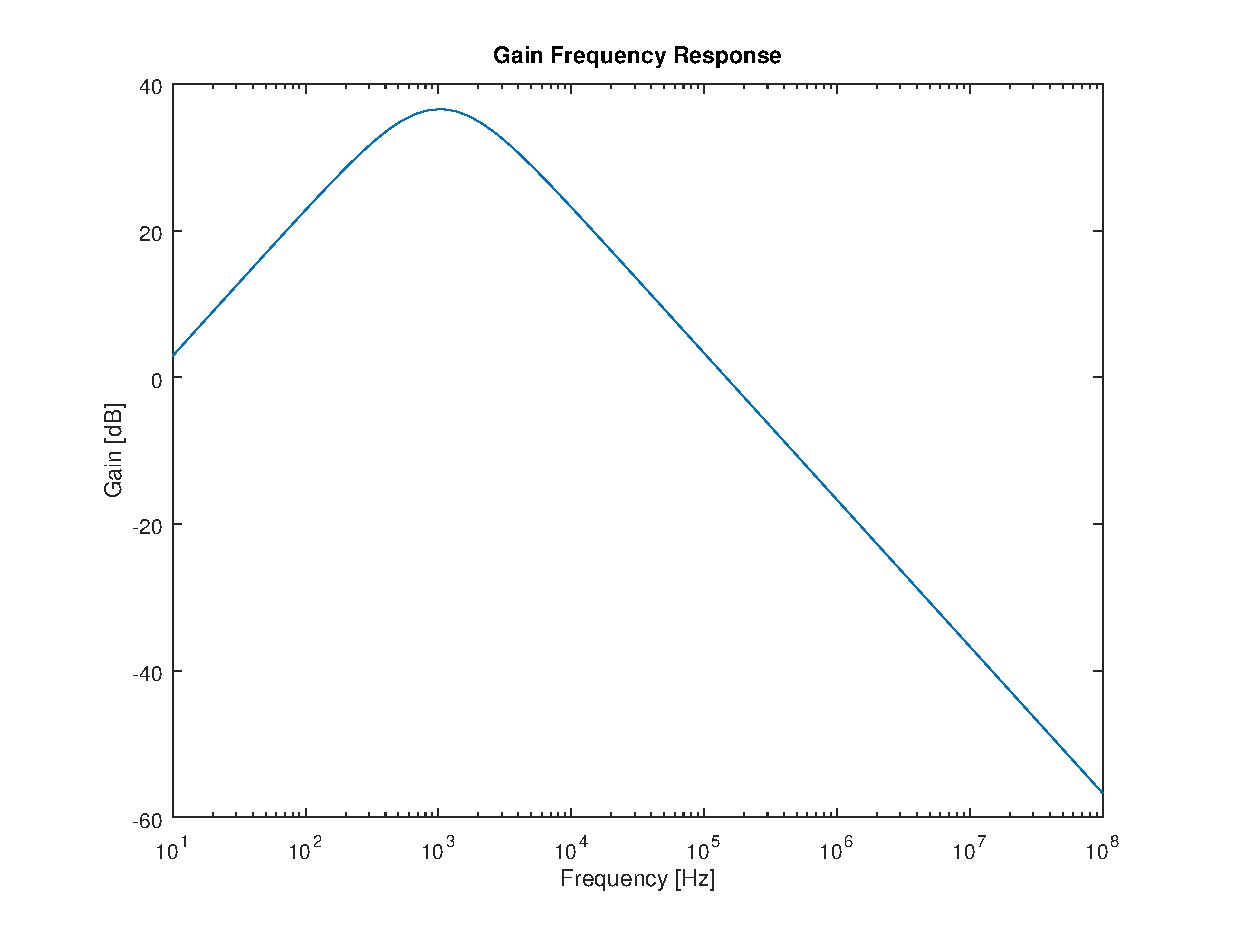
\includegraphics[scale=0.4]{theo_gain_f_response.eps}
    \caption{Theoretical Gain Response}
\end{subfigure}%
\begin{subfigure}{.5\textwidth}
    \centering
    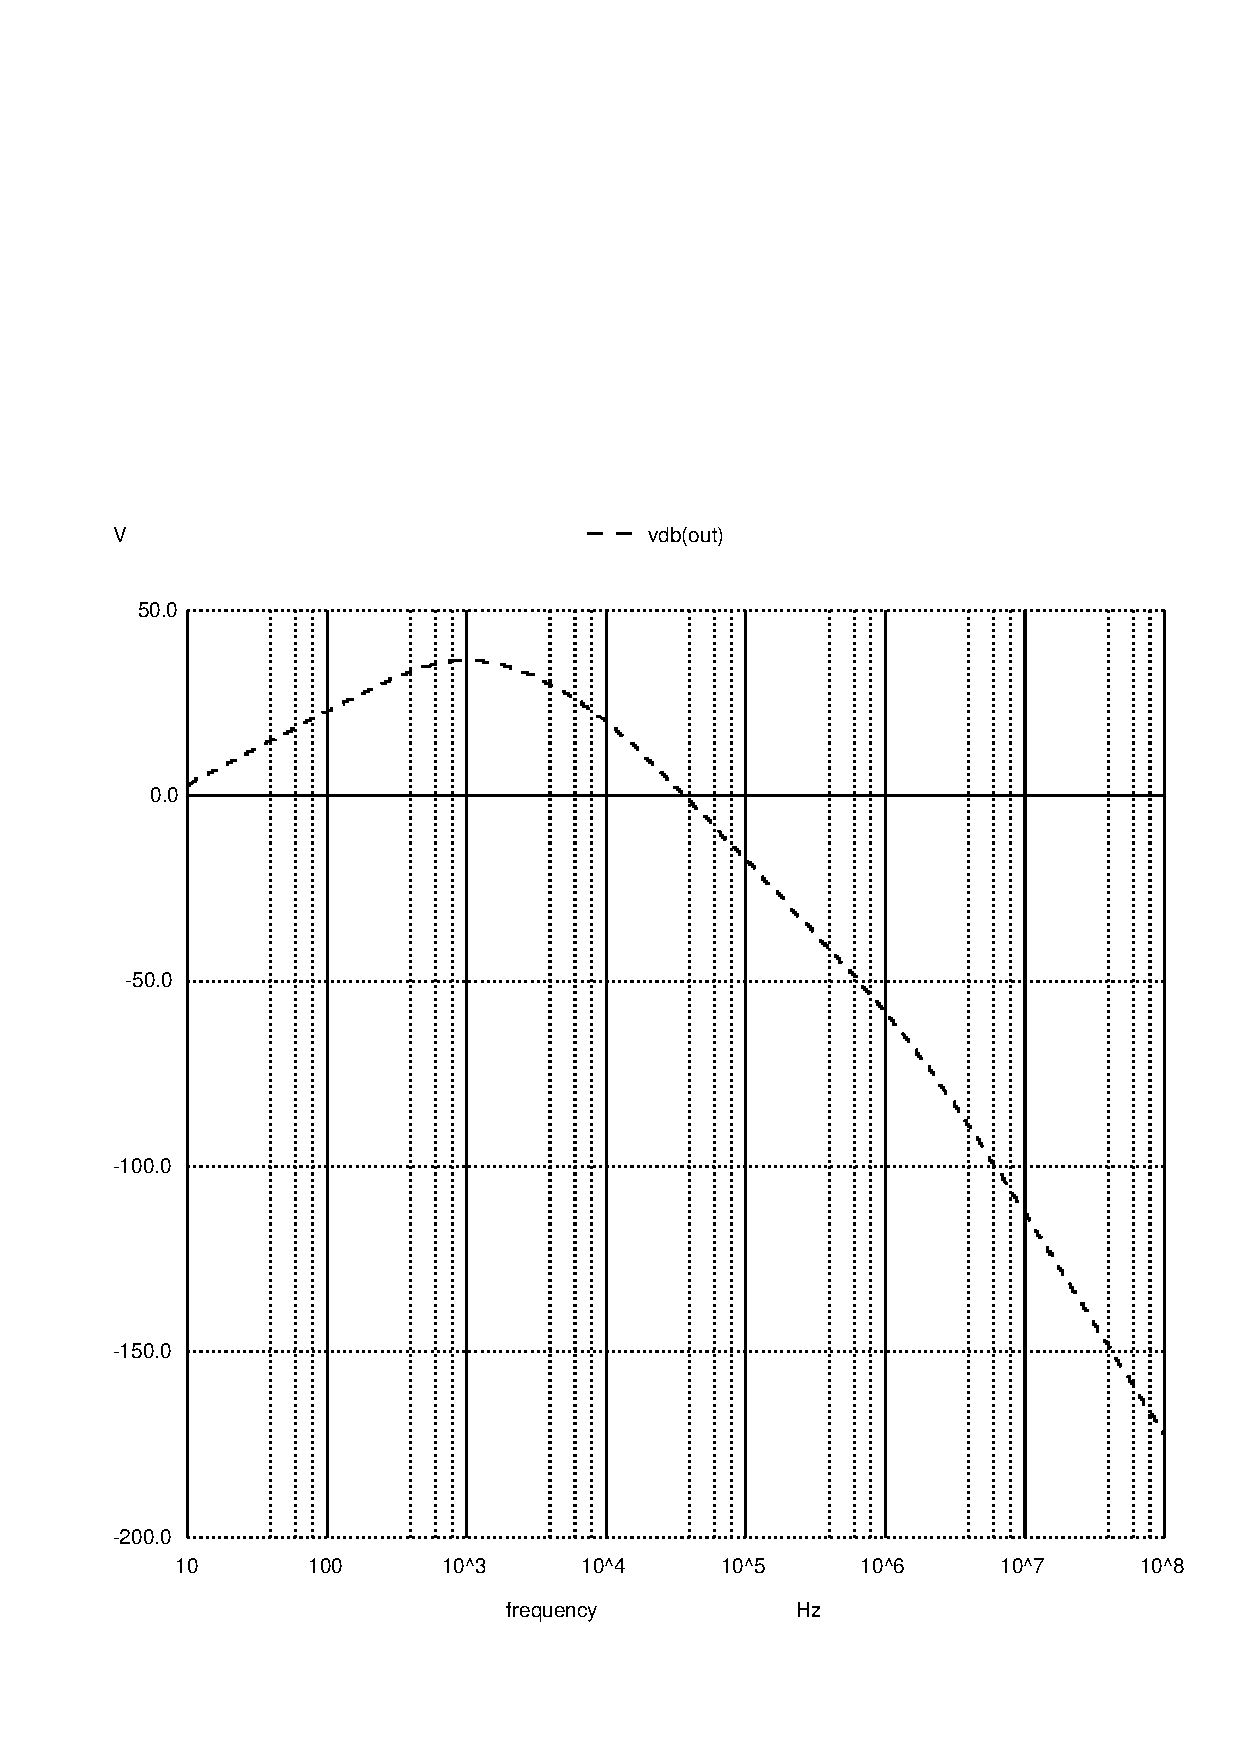
\includegraphics[scale=0.33]{vodb.pdf}
    \caption{Simulation Gain Response}
\end{subfigure}
\begin{subfigure}{.5\textwidth}
    \centering
    \vspace{2.8 cm}
    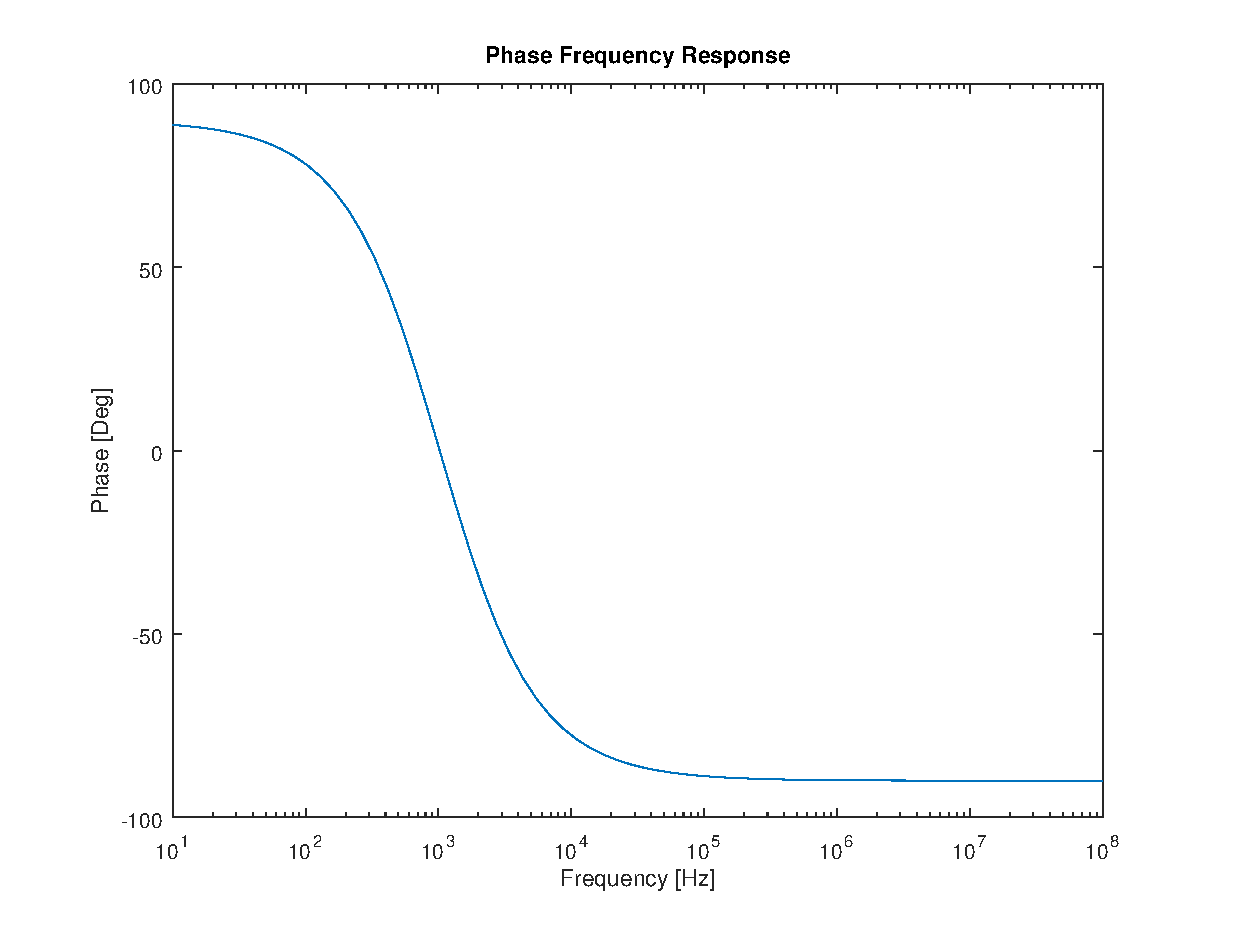
\includegraphics[scale=0.4]{theo_phase_f_response.eps}
    \caption{Theoretical Phase Response}
\end{subfigure}%
\begin{subfigure}{.5\textwidth}
    \centering
    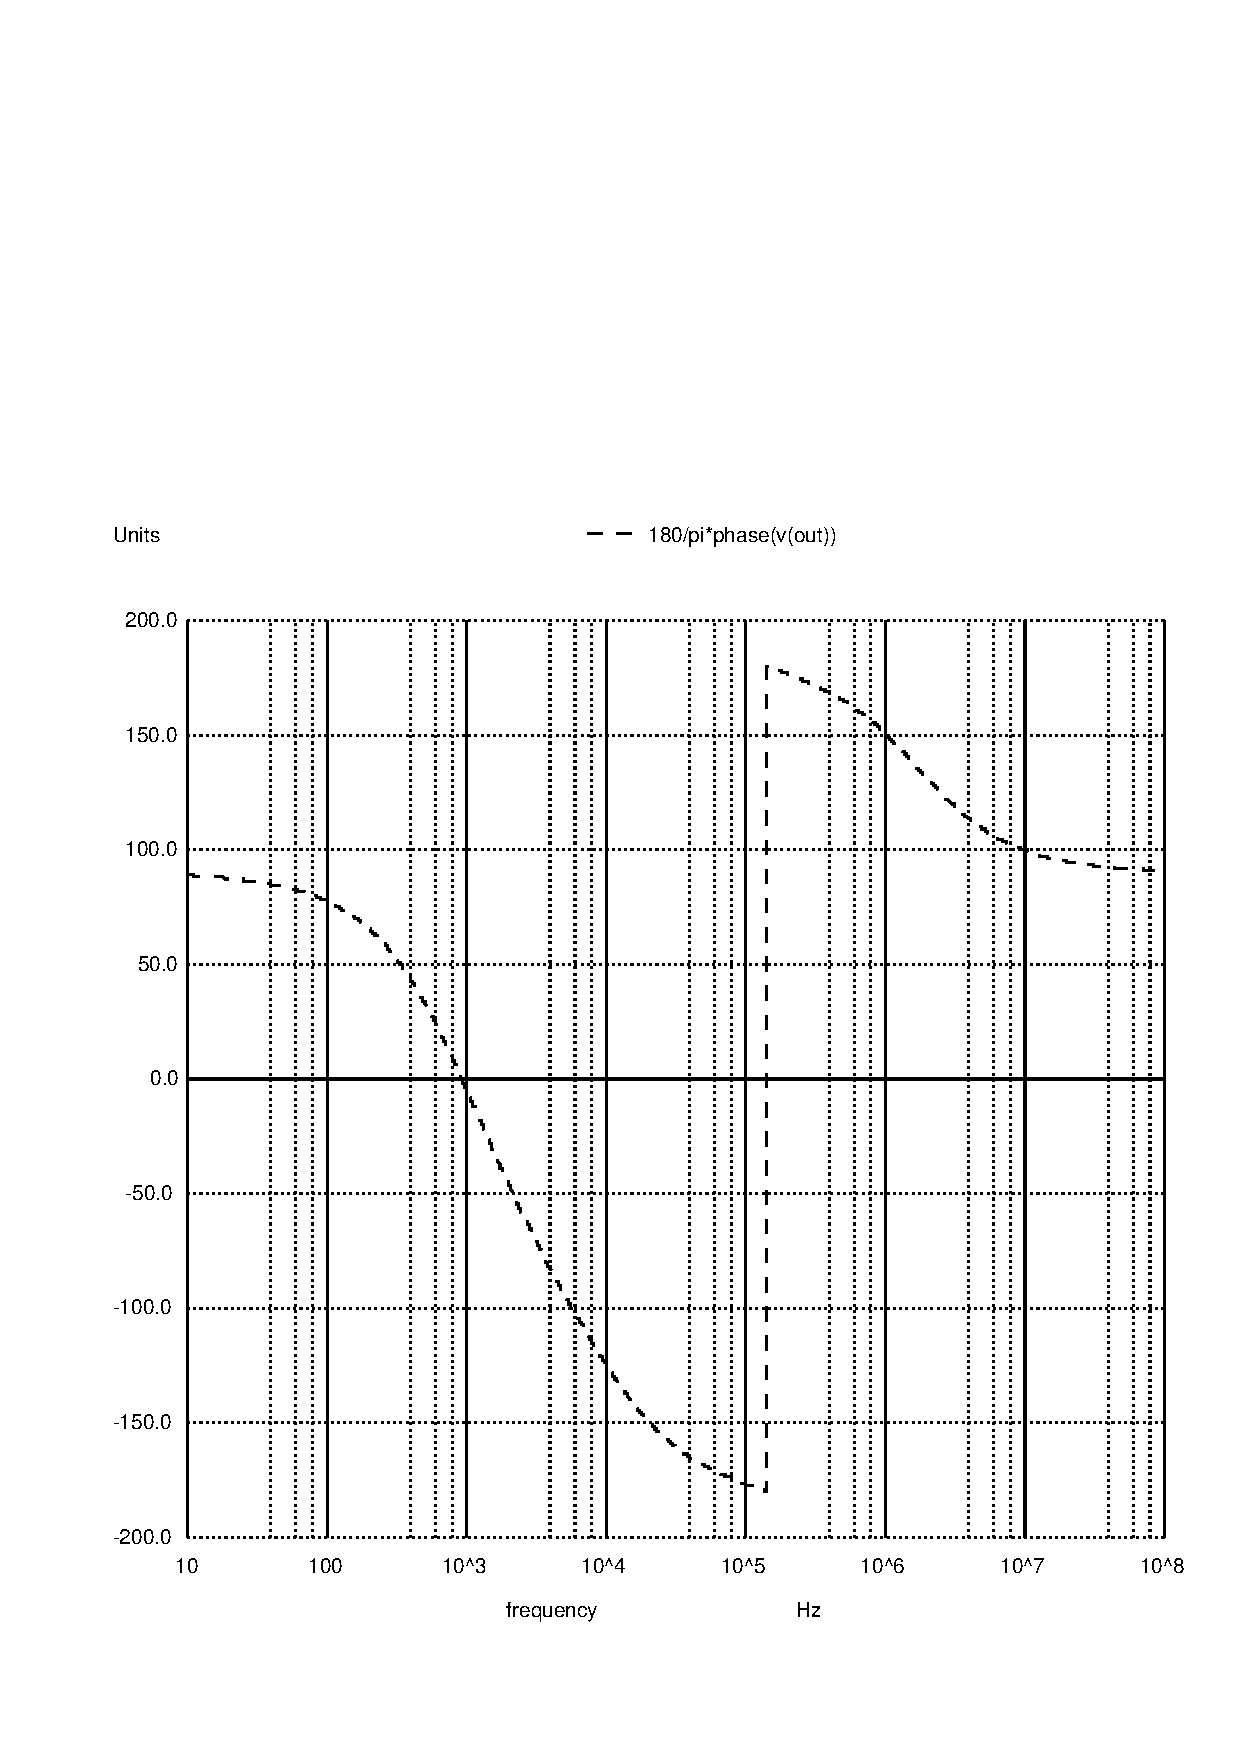
\includegraphics[scale=0.33]{voph.pdf}
    \caption{Simulation Phase Response}
\end{subfigure}
\caption{Frequency Response}
\label{fig:freq_resp}
\end{figure}

\clearpage

\section{Merit Results}
\label{sec:merit}

From the results obtained through the \textit{Ngspice} simulation (see Section \ref{subsec:comparison}) and considering we used the data shown in Section \ref{sec:introduction}, we can compute the price and the merit using the \textit{formulae} given in the lab assignment:

\begin{table}[h]
    \centering
    \begin{tabular}{|l|c|c|}
    \hline
    {\bf Name} & {\bf Value} & {\bf Units} \\ \hline
    AV dev & 32.9164 & \\ \hline
Freq dev & 13.911 & Hz\\ \hline
Cost & 13426.8 & MU\\ \hline
Merit & 1.59048E-06 & \\ \hline

   \end{tabular}
   \caption{Merit Results}
   \label{tab:merit}
\end{table}
